\documentclass[11pt, a4paper]{article}
\usepackage{graphicx, amsmath} % Required for inserting images
\usepackage{algorithm}
\usepackage{algpseudocode}
\usepackage[margin=1in]{geometry}
\begin{document}
\section*{CSCB36 A3: Nena Harsch and Natalia Tabja}
\section*{Question 1 (written by both, verified by both)}
\textbf{Data Structure D is an augmented AVL tree with:} \\
Fields from normal AVL tree: parent, lchild - left child, rchild - right child, bf - balance factor \\
Key field: price \\
Additional field: farea - floor area\\
Augmented field: maxArea - max floor area of the subtree rooted at x and x \\\\
\textbf{Insert(D, x): given a pointer to x} \\
\begin{itemize}
    \item The first phase is to go down the tree from the root and insert the new node as a child of an existing node. We know from AVL insert that this takes $O(log_2n)$ time.
    \item The second phase goes up the tree using the pointers to the parent to update the bf and maxArea simultaneously. We can achieve this by checking the left subtree maxArea, the right subtree maxArea, and the current node's farea. Unlike the AVL insert, we must traverse up until we reach the root because all nodes along the path from the root to the new node could be affected by the new node's farea. Since there are $O(log_2n)$ nodes on the path from the root to the new node, and since updates/ rotations also take constant time (only two nodes are affected in a rotation which need their bf and maxArea updated, and this is constant time), then the total time for insertion is $O(log_2n)$.
\end{itemize}
\textbf{Delete(D, x): given a pointer to x} \\
\begin{itemize}
    \item The first phase is to delete the node. There are three cases.
    \begin{enumerate}
    \item If the node is a leaf, then we just delete that node. Traverse up the tree to the root to rebalance and update like insert.
    \item If x only has one child, then we replace x with the child. Traverse up the tree to the root to rebalance and update like insert.
    \item If x has two children, then we have to find the successor. Once we find the successor, we copy its value into the node x that we are deleting. This "deletes" node x by replacing it with its successor. After copying the successor’s value into x, we now need to delete the successor itself. The successor can either: Be a leaf (remove it without further actions) or have one child (replace the successor with its only child, so that the tree remains connected and valid). Traverse up the tree from the successor to the root to rebalance and update like insert. We must now start at the successor because removing it further down the tree could affect nodes below the node we originally wanted to remove.
    \end{enumerate}
    \item For all the cases, the path from either the deleted node to the root or the successor to the root will be at most height n, so the total time for deletion is $O(log_2n)$.

\end{itemize}
\textbf{MaxArea(D, p):} \\

\begin{algorithm} [H]
\caption{MaxArea(D, p):}
\begin{algorithmic}[1]
\State \textbf{Input:} the root of the augmented AVL described above \( D \), price \( p \)
\State \textbf{Output:} Return the maximum floor area of listings whose price is at most $p$. If no listing has price at most $p$, then return $-1$.
\\

\If{$D = NIL$}
    \State return -1
\ElsIf{$D.\text{price} > p$}
        \State \textbf{return} MaxArea($D.\text{lchild}$, $p$)
\Else
        \State $checkl \gets \text{MaxArea}(D.\text{lchild}, p)$
        \State $checkr \gets \text{MaxArea}(D.\text{rchild}, p)$
        \State \textbf{return} $\max(checkl, checkr, D.farea)$
\EndIf

\end{algorithmic}
\end{algorithm}

\section*{Example of the Data Structure}

In order to illustrate how our data structure works, we will consider the following simple set of listings: 
\begin{itemize}
    \item Listing 1: Price = 300k, Area = 120 sqm
    \item Listing 2: Price = 200k, Area = 90 sqm
    \item Listing 3: Price = 400k, Area = 150 sqm
    \item Listing 4: Price = 100k, Area = 70 sqm
\end{itemize}

We now insert each listing into the AVL tree.

\begin{itemize}
    \item \textbf{Step 1: Insert Listing 1 (300k, 120 sqm):} This becomes the root of the tree since it is the first listing inserted.
    \item \textbf{Step 2: Insert Listing 2 (200k, 90 sqm):} Since 200k $<$  300k, this node becomes the left child of the root. The tree is still balanced.
    \item \textbf{Step 3: Insert Listing 3 (400k, 150 sqm):} Since 400k $>$ 300k, this node becomes the right child of the root. The root’s maxArea field is updated to 150 sqm since the right subtree contains a larger area than the root’s own area. The tree remains balanced so no rotations are required.
    \item \textbf{Step 4: Insert Listing 4 (100k, 70 sqm):} Since 100k $<$ 200k, this node becomes the left child of the node with price 200k. The tree remains balanced, and the maxArea fields of the left subtree remain unchanged as the largest area there is still 90 sqm.
\end{itemize}

\begin{figure}
    \centering
    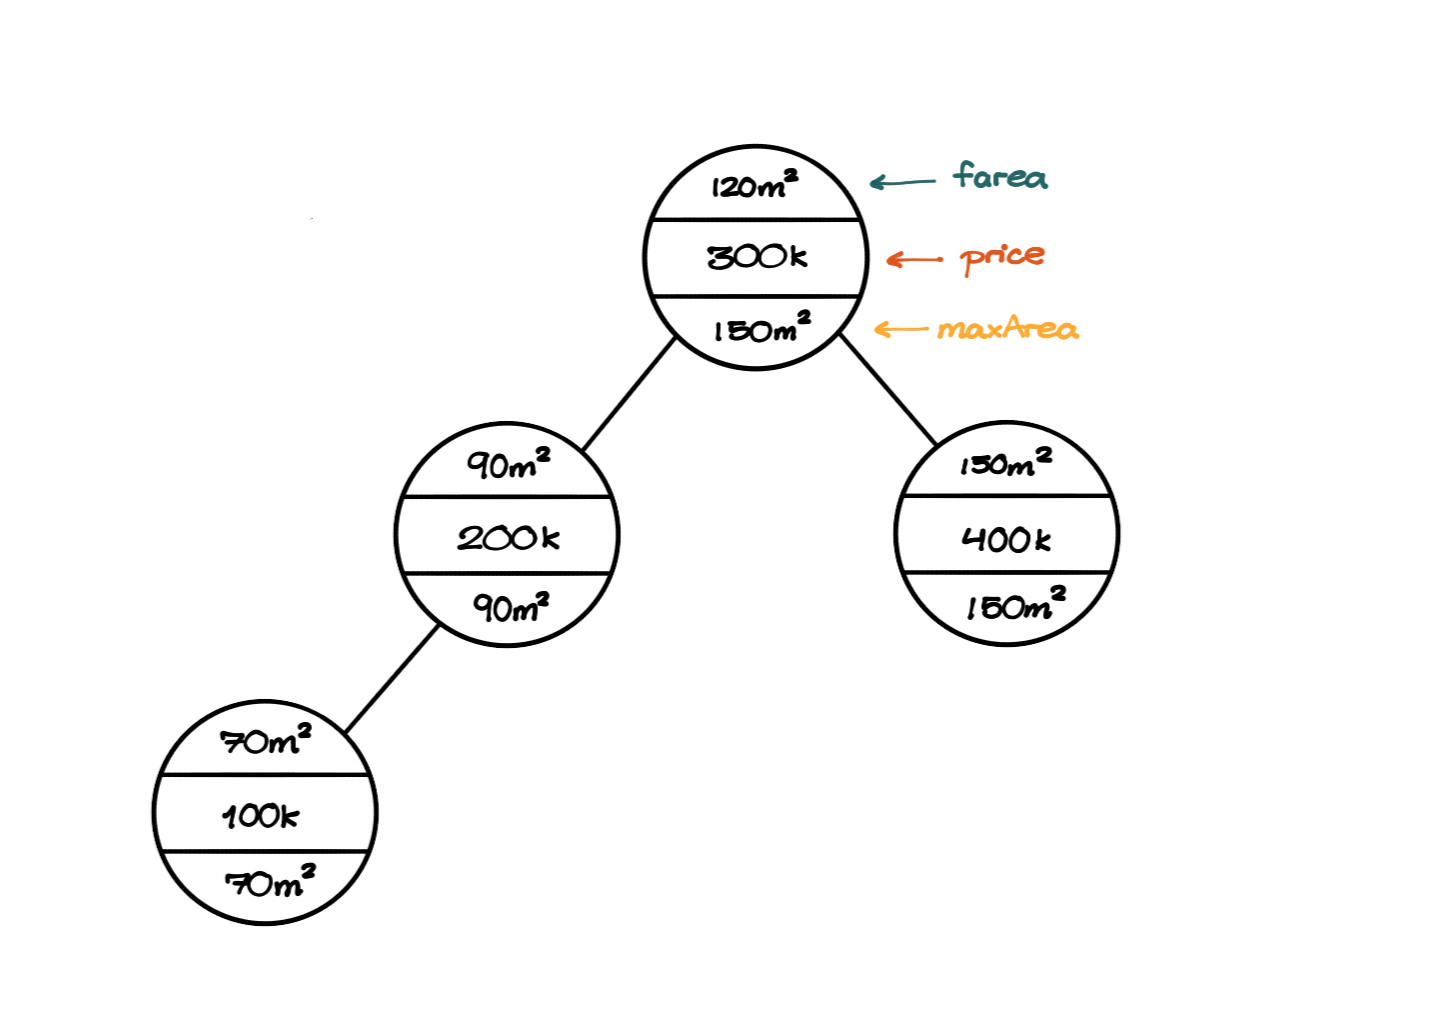
\includegraphics[width=0.5\linewidth]{data_struct_a3.jpeg}
    \caption{Augmented AVL Tree after all Insertions}
    \label{fig:enter-label}
\end{figure}

\textbf{Example Method Calls:}
\begin{itemize}
    \item If we call \texttt{MaxArea(D, 350)}, the function will return 120 sqm, as the largest floor area of listings with price \( \leq 350k \) is the area of the root node (300k, 120 sqm).
    \item If we call \texttt{MaxArea(D, 200)}, the function will return 90 sqm, as the largest floor area of listings with price \( \leq 200k \) is the area of the node with price 200k.
\end{itemize}


\section*{Question 2 (written by Nena, verified by Natalia)}
\textbf{Data Structure S is an augmented AVL tree with:} \\
Fields from normal AVL tree: parent, lchild - left child, rchild - right child, bf - balance factor \\
Key field: id \\
Augmented field: rPresent - True if there exists a node in the subtree rooted at x that is ready (including x) \\\\
\textbf{NewThread(t)} \\
\begin{itemize}
    \item The first phase it to go down the tree from the root and insert the new node as a child of an existing node. We know from AVL insert that this takes $O(log_2n)$ time.
    \item The second phase goes up the tree using the pointers to the parent to update the bf and rPresent simultaneously. Unlike the AVL insert, we must traverse up until we reach the root because all nodes along the path from the root to the new node could be affected by the new node's farea. Since there are $O(log_2n)$ nodes on the path from the root to the new node, and since updates/ rotations also take constant time (only two nodes are affected in a rotation which need their bf and rPresent updated, and this is constant time), then the total time for insertion of a new thread is $O(log_2n)$.
\end{itemize}
\textbf{Find(i)} \\
\begin{itemize}
    \item This is just a simple search like the AVL tree. Since all id's are unique, once we find the id that matches we are done. If we do not find it, then we return -1.
\end{itemize}
\textbf{Completed(i)} \\
\begin{itemize}
    \item First, we need to use Find(i) to see if there exists a thread with id i. If there is, then we can use a delete function to delete the thread i. There are three cases:
    \begin{enumerate}
    \item If the node is a leaf, then we just delete that node. Traverse up the tree to the root to rebalance and update like NewThread.
    \item If x only has one child, then we replace x with the child. Traverse up the tree to the root to rebalance and update like NewThread.
    \item If x has two children, then we have to find the successor. Once we find the successor, we copy its value into the node x that we are deleting. This "deletes" node x by replacing it with its successor. After copying the successor’s value into x, we now need to delete the successor itself. The successor can either: Be a leaf (remove it without further actions) or have one child (replace the successor with its only child, so that the tree remains connected and valid). Traverse up the tree from the successor to the root to rebalance and update like NewThread. We must now start at the successor because removing it further down the tree could affect nodes below the node we originally wanted to remove.
    \end{enumerate}
    \item For all the cases, the path from either the deleted node to the root or the successor to the root will be at most height $log_2n$, so the total time for deletion is $O(log_2n)$.
\end{itemize}
\textbf{ChangeStatus(i, stat)}

\begin{algorithm} [H]
\caption{ChangeStatus(i, stat):}
\begin{algorithmic}[1]
\State \textbf{Input:} the thread's id we are looking for \( i \), the new status \( stat \)
\State \textbf{Output:} Return -1 if S does not have a thread $t = (i, -)$
\\
    \State $t \gets \text{Find}(i)$
    \If{$t \neq \text{NIL}$}
        \State $t.\text{status} \gets \text{stat}$
        \While{$t \neq \text{NIL}$}
            \If {$t.\text{status} = \text{R}$ \textbf{or} $t.\text{lchild.rPresent} = \text{True}$ \textbf{or} $t.\text{rchild.rPresent} = \text{True}$}
                \State $t.\text{rPresent} \gets \text{True}$
            \EndIf
            \State $t \gets t.\text{parent}$
        \EndWhile
    \Else
        \State \textbf{return} $-1$
    \EndIf

\end{algorithmic}
\end{algorithm}
\textbf{ScheduleNext()}

\begin{algorithm} [H]
\caption{ScheduleNext():}
\begin{algorithmic}[1]
\State \textbf{Input:}
\State \textbf{Output:} Return -1 if S does not have a thread whose status is R
\\
    \If{$S.rPresent \neq NIL$}
        \While{$S \neq \text{NIL}$}
            \If {$S.lchild \neq NIL$ and $S.lchild.rPresent$}
                \State $S \gets S.lchild$
            \ElsIf {$S.status \neq R$}
                \State return $S$
            \Else
                \State $S \gets S.rchild$
            \EndIf
        \EndWhile
    \Else
        \State \textbf{return} $-1$
    \EndIf

\end{algorithmic}
\end{algorithm}

\section*{Question 3 (written by Natalia, verified by Nena)}

\textbf{Part a) Algorithm Description:}
\begin{enumerate}
    \item \textbf{Hashing:} First, all numbers in \( L \) will be passed through a hash function and stored in a hash map along with their associated frequencies in \( L \). E.g. \(h(x) = x \mod m\), with \(m\) = size of hash table, and \(m\) being a prime number. Whenever a new integer is added to the map, if the key corresponding to that integer already exists, then its frequency will just be incremented by 1. Otherwise, it will be added to the map with a frequency of 1.
    \item \textbf{Grouping integers by frequency:} Next, we will create an array of lists where each index corresponds to a possible frequency, and the list at that index will contain all the numbers that appear in \( L \) with that frequency. For instance, every integer that occurs in \( L \) twice would be stored in the list at the second index of this array.
    \item \textbf{Concatenating lists:} In order to get a single list to output, we must concatenate the lists in such a way that it's ordered from highest to lowest frequency. This can be achieved by traversing the array in the previous step from end to start, collecting the integers from the list at each index (if it exists) into a new list. This ensures that the integers are ordered by their frequency in non-increasing order. If multiple integers have the same frequency, they can appear in any order. The resulting list contains the distinct integers from \( L \) sorted in non-increasing order of their frequencies. We return this list.
\end{enumerate}

\textbf{Part b) Time Complexity Analysis:}
\begin{enumerate}
    \item \textbf{Hashing:} The hash map allows inserting elements and updating frequencies in \( O(1) \) average time due to hashing. When collisions occur, we chain the values together by updating frequencies instead of adding to a linked list to avoid having to traverse a list for each integer in linear time when grouping the integers by frequency. Under SUHA, this assumption would prevent each entry for being overloaded, but because we are just storing the frequency it is not needed explicitly. Therefore, for \( n \) elements in \( L \), building the frequency map takes \( O(n) \) time.
    \item \textbf{Grouping integers by frequency:} For each element in the hash table, to retrieve the value and frequency takes \( O(1) \) time. Then, placing the value into the index of the frequency also takes \( O(1) \)  time because we will insert it into the beginning of the list which is \( O(1) \) time. Therefore,  this operation also takes \( O(n) \) time because the number of elements in the hash map is proportional to the number of elements in \( L \), and placing each integer into its respective list takes constant time.
    \item \textbf{Concatenating lists:} The number of possible frequencies is at most \( n \). Since we are iterating through the frequencies in decreasing order (from \( n \) down to 1), and simply concatenating lists of integers, this step also takes \( O(n) \) time (at most n concatenations).
\end{enumerate}

\textbf{Part c) Worst-case Time Complexity:}
In the worst case:
\begin{itemize}
    \item \textbf{Hashing:} If the hash function behaves poorly and results in a high number of collisions, the operations insert and update on the hash map would remain \( O(1) \) the same since we chain the values together by updating frequencies instead of adding to a linked list. This avoids the hash table becoming a single linked list. But, we would still need to look through the entire hash table to lookup when inserting them into a list by frequency. Since we still map \( n \) elements in \( L \), building the frequency map takes \( O(n) \) time.
    \item \textbf{Grouping by Frequency and Sorting:} These steps remain \( O(n) \) because regardless of how the integers are distributed, we would still need to look through the entire hash table to build the frequency buckets, the number of frequency buckets is no more than \( n \), and iterating over the buckets still takes linear time.
\end{itemize}


\end{document}